\documentclass[11pt,a4paper]{article}

\usepackage[margin=1.75cm]{geometry}
\usepackage{fontspec}
\usepackage{microtype}
\usepackage{amsmath}
\usepackage{array}
\usepackage{booktabs}
\usepackage{tabularx}
\usepackage{enumitem}
\usepackage{fancyvrb}
\usepackage[most]{tcolorbox}
\usepackage{tikz}
\usetikzlibrary{
  arrows.meta,
  backgrounds,
  calc,
  fit,
  matrix,
  positioning,
  shapes.geometric
}
\usepackage[
  colorlinks=true,
  linkcolor=blue!50!black,
  urlcolor=blue!50!black
]{hyperref}

\setmainfont{DejaVu Sans}
\setsansfont{DejaVu Sans}
\setmonofont{DejaVu Sans Mono}

\definecolor{ink}{HTML}{29251F}
\definecolor{muted}{HTML}{6D665D}
\definecolor{paper}{HTML}{FAF8F2}
\definecolor{line}{HTML}{CEC6B8}
\definecolor{gold}{HTML}{8A6527}
\definecolor{goldlight}{HTML}{F4E7C2}
\definecolor{blue}{HTML}{2E6F9E}
\definecolor{bluelight}{HTML}{DCECF7}
\definecolor{green}{HTML}{3B7D57}
\definecolor{greenlight}{HTML}{DFF0E6}
\definecolor{red}{HTML}{A33B35}
\definecolor{redlight}{HTML}{F7E1DF}
\definecolor{purple}{HTML}{74518E}
\definecolor{purplelight}{HTML}{EDE2F3}
\definecolor{greycell}{HTML}{EEEAE1}

\color{ink}
\pagecolor{paper}
\setlength{\parindent}{0pt}
\setlength{\parskip}{7pt}
\setlist[itemize]{leftmargin=1.4em,itemsep=4pt,topsep=3pt}
\setlist[enumerate]{leftmargin=1.6em,itemsep=4pt,topsep=3pt}
\renewcommand{\arraystretch}{1.22}

\newcommand{\op}[1]{\texttt{\bfseries #1}}
\newcommand{\reg}[1]{\textsf{\bfseries #1}}
\newcommand{\Fib}[1]{F_{#1}}
\newcommand{\yes}{\textcolor{green}{\bfseries YES}}
\newcommand{\no}{\textcolor{red}{\bfseries NO}}

\newtcolorbox{plainbox}[1][]{
  enhanced,
  breakable,
  colback=white,
  colframe=line,
  boxrule=0.7pt,
  arc=2mm,
  left=3mm,
  right=3mm,
  top=2.5mm,
  bottom=2.5mm,
  #1
}

\newtcolorbox{keybox}[1][]{
  enhanced,
  breakable,
  colback=goldlight!55!white,
  colframe=gold,
  boxrule=0.8pt,
  arc=2mm,
  left=3mm,
  right=3mm,
  top=2.5mm,
  bottom=2.5mm,
  #1
}

\newtcolorbox{bluebox}[1][]{
  enhanced,
  breakable,
  colback=bluelight!55!white,
  colframe=blue,
  boxrule=0.8pt,
  arc=2mm,
  left=3mm,
  right=3mm,
  top=2.5mm,
  bottom=2.5mm,
  #1
}

\newtcolorbox{warningbox}[1][]{
  enhanced,
  breakable,
  colback=redlight!55!white,
  colframe=red,
  boxrule=0.8pt,
  arc=2mm,
  left=3mm,
  right=3mm,
  top=2.5mm,
  bottom=2.5mm,
  #1
}

\tikzset{
  flow/.style={
    -{Latex[length=3mm]},
    line width=1.1pt,
    draw=blue,
    rounded corners=2pt
  },
  dataflow/.style={
    -{Latex[length=3mm]},
    line width=1.2pt,
    draw=green
  },
  arrowlabel/.style={
    fill=paper,
    inner sep=1.2pt,
    font=\small,
    align=center
  },
  room/.style={
    draw=ink,
    fill=white,
    very thick,
    rounded corners=2pt,
    minimum height=1.5cm,
    align=center
  },
  register/.style={
    draw=gold,
    fill=goldlight,
    rounded corners=2pt,
    minimum width=2.65cm,
    minimum height=1.15cm,
    align=center
  },
  process/.style={
    draw=blue,
    fill=bluelight,
    rounded corners=2pt,
    minimum width=2.35cm,
    minimum height=1cm,
    align=center
  },
  decision/.style={
    diamond,
    aspect=2.1,
    draw=purple,
    fill=purplelight,
    very thick,
    align=center,
    inner sep=1.5pt
  },
  opcell/.style={
    draw=line,
    fill=greycell,
    minimum width=6.4mm,
    minimum height=6.4mm,
    inner sep=0pt,
    font=\ttfamily\bfseries
  },
  initcell/.style={
    opcell,
    fill=goldlight,
    draw=gold
  },
  loopcell/.style={
    opcell,
    fill=bluelight,
    draw=blue
  },
  exitcell/.style={
    opcell,
    fill=greenlight,
    draw=green
  }
}

\hypersetup{
  pdftitle={Fibonacci in Littleman: a picture-first guide},
  pdfauthor={team wheezards / Codex},
  pdfsubject={An illustrated explanation of a one-man Littleman program}
}

\begin{document}

\begin{titlepage}
  \vspace*{1.0cm}

  {\color{gold}\rule{\textwidth}{2.2pt}}

  \vspace{0.8cm}
  {\sffamily\bfseries\fontsize{34}{39}\selectfont
    Fibonacci in Littleman\par}
  \vspace{0.25cm}
  {\sffamily\fontsize{20}{25}\selectfont
    A picture-first guide for a complete beginner\par}

  \vspace{0.8cm}

  \begin{keybox}
    \centering
    \Large
    The entire idea is this:
    \[
      \boxed{\reg{A}=\Fib{k}}
      \qquad
      \boxed{\reg{B}=\Fib{k+1}}
      \qquad
      \boxed{\reg{BP}=n-k}
    \]
    One lap changes \(k\) into \(k+1\). After \(n\) laps,
    \(\reg{A}=\Fib{n}\), so the man sends \reg{A} to the output.
  \end{keybox}

  \vfill

  \begin{center}
  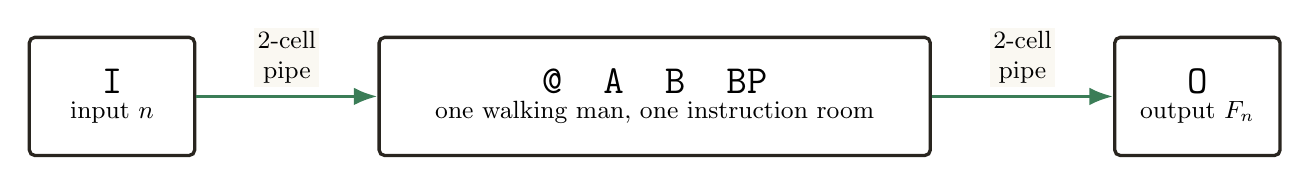
\begin{tikzpicture}[node distance=1.0cm]
    \node[room, minimum width=2.1cm] (input) {
      \Large\texttt{I}\\[-1mm]
      \small input \(n\)
    };
    \node[room, minimum width=7cm, right=2.3cm of input] (worker) {
      \Large\texttt{@\quad A\quad B\quad BP}\\[-1mm]
      \small one walking man, one instruction room
    };
    \node[room, minimum width=2.1cm, right=2.3cm of worker] (output) {
      \Large\texttt{O}\\[-1mm]
      \small output \(\Fib{n}\)
    };
    \draw[dataflow] (input) --
      node[arrowlabel, midway, above=1mm]{2-cell\\pipe} (worker);
    \draw[dataflow] (worker) --
      node[arrowlabel, midway, above=1mm]{2-cell\\pipe} (output);
  \end{tikzpicture}
  \end{center}

  \vfill

  \begin{plainbox}
    \textbf{What this guide assumes:} nothing beyond ordinary addition.
    It explains what the rooms are, what every used character means,
    where the man walks, what is in each register after every important
    operation, why the loop stops, and why the answer is correct.
  \end{plainbox}

  \vspace{0.8cm}
  {\small
    The teaching program and both compact variants were validated against
    eight cases, \(0\le n\le92\), with the repository Littleman simulator.
    All arithmetic is signed 64-bit.
    \hfill 2026-07-31
  }
\end{titlepage}

\tableofcontents
\clearpage

\section{First: what kind of ``computer'' is this?}

Do not imagine that the little man must remember the entire computation in
his head. Imagine a tiny CPU walking over its own program:

\begin{center}
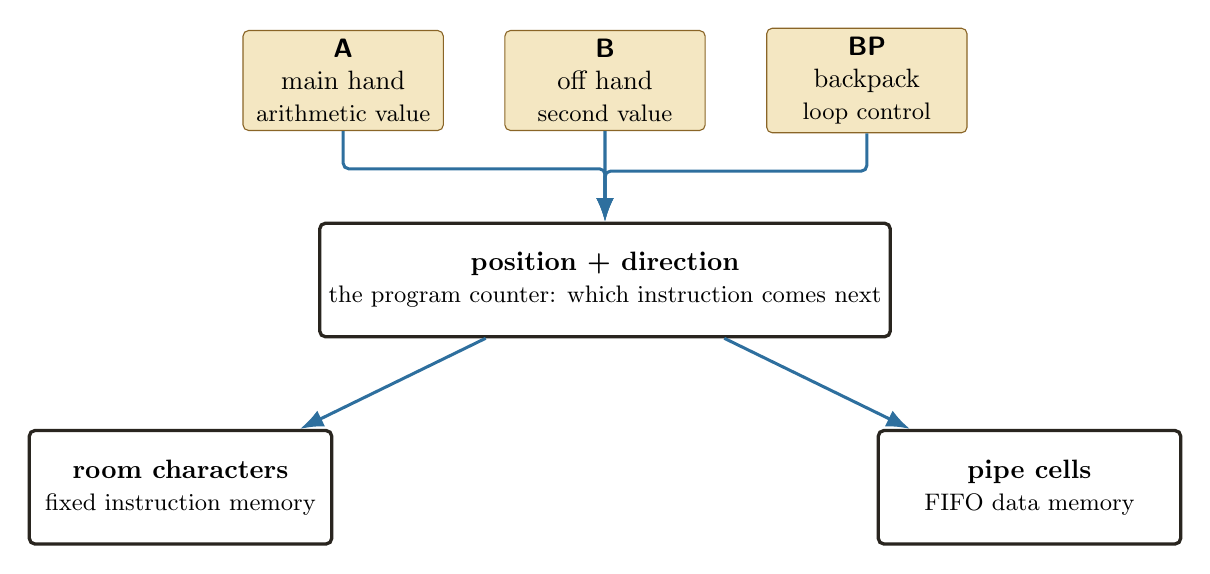
\begin{tikzpicture}[node distance=7mm and 8mm, scale=0.96, transform shape]
  \node[register] (a) {\reg{A}\\main hand\\\small arithmetic value};
  \node[register, right=of a] (b) {\reg{B}\\off hand\\\small second value};
  \node[register, right=of b] (bp) {\reg{BP}\\backpack\\\small loop control};

  \node[room, below=12mm of b, minimum width=5.4cm] (position) {
    \textbf{position + direction}\\
    \small the program counter: which instruction comes next
  };

  \node[room, below left=12mm and -2mm of position, minimum width=4cm] (grid) {
    \textbf{room characters}\\
    \small fixed instruction memory
  };
  \node[room, below right=12mm and -2mm of position, minimum width=4cm] (pipes) {
    \textbf{pipe cells}\\
    \small FIFO data memory
  };

  \draw[flow] (a.south) -- ($(a.south)+(0,-5mm)$) -| (position.north);
  \draw[flow] (b.south) -- (position.north);
  \draw[flow] (bp.south) -- ($(bp.south)+(0,-5mm)$) -| (position.north);
  \draw[flow] (position) -- (grid);
  \draw[flow] (position) -- (pipes);
\end{tikzpicture}
\end{center}

\begin{keybox}
  \textbf{The hands are working registers, not total memory.}
  A normal CPU can process a large file with only a few registers because
  it handles one piece at a time and stores the rest elsewhere. Littleman
  works the same way. In this Fibonacci program there is no large data set:
  two consecutive numbers are sufficient, so \reg{A} and \reg{B} are all
  the data memory we need.
\end{keybox}

\subsection{One tick}

Time advances in discrete ticks. For our program, the useful mental model is:

\begin{enumerate}
  \item Values in pipes move one cell toward their destination.
  \item The man executes the character under his feet.
  \item Unless blocked or halted, he moves one cell in his current direction.
\end{enumerate}

He begins on \op{@} facing right. A blank space is a real instruction:
``do nothing, then keep walking.''

\section{The problem}

We choose the standard Fibonacci convention:
\[
  \Fib{0}=0,\qquad
  \Fib{1}=1,\qquad
  \Fib{n}=\Fib{n-1}+\Fib{n-2}\quad(n\ge2).
\]

The machine receives one integer \(n\), computes \(\Fib{n}\), emits that one
integer, and halts. We restrict \(0\le n\le92\), because \(\Fib{92}\) is the
largest Fibonacci answer that fits in a positive signed 64-bit integer.

\begin{center}
\begin{tabular}{c|rrrrrrrrrrr}
  \(n\) & 0&1&2&3&4&5&6&7&8&9&10\\
  \midrule
  \(\Fib{n}\) & 0&1&1&2&3&5&8&13&21&34&55
\end{tabular}
\end{center}

\begin{bluebox}
  \textbf{Why this is a perfect first example.}
  Fibonacci needs a loop, arithmetic, input, output, and all three registers,
  but it does \emph{not} need a pipe ring or a second working man. We can see
  the core execution model without extra machinery.
\end{bluebox}

\section{The complete program}

\begin{plainbox}[title={Copyable \texttt{.man} source}]
\VerbatimInput[
  fontsize=\small,
  frame=none,
  commandchars=\\\{\}
]{docs/littleman_fibonacci.man}
\end{plainbox}

The parser sees three rooms:

\begin{itemize}
  \item \texttt{|I|}: the special input room; it contains no man.
  \item the large middle rectangle: the only instruction room; it contains
        one \op{@}, hence one man.
  \item \texttt{|O|}: the special output room; it contains no man.
\end{itemize}

The \texttt{>>} pairs are two-cell pipes. The left pipe carries \(n\) into
the worker. The right pipe carries the final answer out.

\subsection{The same program as a map}

\begin{center}
\resizebox{\textwidth}{!}{%
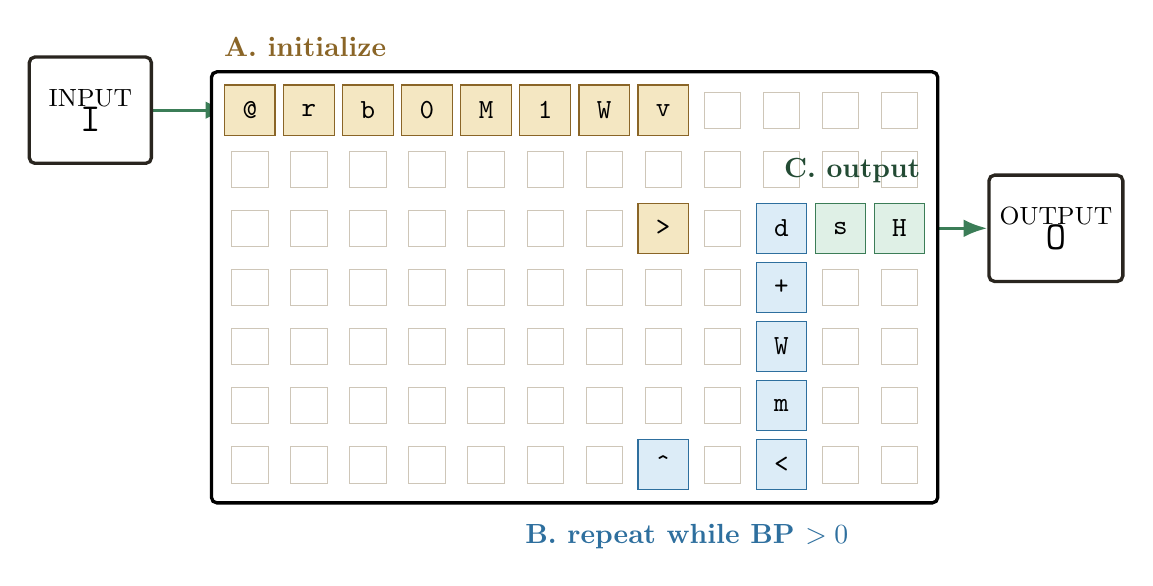
\begin{tikzpicture}[x=0.75cm,y=-0.75cm]
  % Main room and faint cell grid.
  \draw[very thick, fill=white, rounded corners=2pt]
    (0.35,0.35) rectangle (12.65,7.65);
  \foreach \x in {1,...,12}{
    \foreach \y in {1,...,7}{
      \draw[line, very thin]
        ($(\x,\y)+(-0.31,-0.31)$) rectangle
        ($(\x,\y)+(0.31,0.31)$);
    }
  }

  % I/O rooms.
  \node[room, minimum width=1.55cm, minimum height=1.35cm]
    (in) at (-1.7,1) {\small INPUT\\[-1mm]\Large\texttt{I}};
  \node[room, minimum width=1.7cm, minimum height=1.35cm]
    (out) at (14.65,3) {\small OUTPUT\\[-1mm]\Large\texttt{O}};

  % Execution paths go behind the operation cells.
  \begin{scope}[on background layer]
    \draw[-{Latex[length=2.3mm]}, line width=2.2pt, draw=gold!65,
      rounded corners=3pt]
      (1,1) -- (8,1) -- (8,3) -- (9.7,3);
    \draw[-{Latex[length=2.3mm]}, line width=2.2pt, draw=blue!70,
      rounded corners=3pt]
      (10,3.25) -- (10,7) -- (8,7) -- (8,3.08) -- (9.68,3.08);
    \draw[-{Latex[length=2.3mm]}, line width=2.2pt, draw=green!75!black]
      (10.3,3) -- (12,3);
    \draw[dataflow] (in.east) -- (0.65,1);
    \draw[dataflow] (12.35,3) -- (out.west);
  \end{scope}

  % Initialization cells.
  \node[initcell] at (1,1) {@};
  \node[initcell] at (2,1) {r};
  \node[initcell] at (3,1) {b};
  \node[initcell] at (4,1) {0};
  \node[initcell] at (5,1) {M};
  \node[initcell] at (6,1) {1};
  \node[initcell] at (7,1) {W};
  \node[initcell] at (8,1) {v};
  \node[initcell] at (8,3) {>};

  % Loop/exit cells.
  \node[loopcell] at (10,3) {d};
  \node[exitcell] at (11,3) {s};
  \node[exitcell] at (12,3) {H};
  \node[loopcell] at (10,4) {+};
  \node[loopcell] at (10,5) {W};
  \node[loopcell] at (10,6) {m};
  \node[loopcell] at (10,7) {<};
  \node[loopcell] at (8,7) {\string^};

  % Labels.
  \node[font=\bfseries, text=gold, anchor=south west]
    at (0.4,0.25) {A. initialize};
  \node[font=\bfseries, text=blue, anchor=north west]
    at (5.5,7.85) {B. repeat while BP \(>0\)};
  \node[font=\bfseries, text=green!60!black, anchor=south]
    at (11.2,2.4) {C. output};
\end{tikzpicture}%
}
\end{center}

\begin{plainbox}
  \textbf{Read the colors in order:}
  \textcolor{gold}{gold} runs once;
  \textcolor{blue}{blue} is the repeated lap;
  \textcolor{green}{green} runs once at the end.
  The arrows show the man's route, not the movement of numbers in a pipe.
\end{plainbox}

\clearpage
\section{Every character used}

\begin{center}
\begin{tabularx}{\textwidth}{>{\centering\arraybackslash}p{1.2cm}
                             >{\raggedright\arraybackslash}p{3.2cm}
                             X}
  \toprule
  \textbf{Cell} & \textbf{Name} & \textbf{Exact effect when executed}\\
  \midrule
  \op{@} & spawn & The man starts here facing right. Later it behaves like
                    a blank cell.\\
  \op{r} & receive & Take one value from the nearest incoming pipe and put it
                     in \reg{A}. Wait here if no value has arrived.\\
  \op{b} & backpack write & Copy \reg{A} into \reg{BP}. \reg{A} is unchanged.\\
  \op{0}, \op{1} & constants & Replace \reg{A} with that digit.\\
  \op{M} & copy hand & Copy \reg{A} into \reg{B}. \reg{A} is unchanged.\\
  \op{W} & swap hands & Exchange \reg{A} and \reg{B}.\\
  \op{+} & add & Set \(\reg{A}\leftarrow\reg{A}+\reg{B}\).
                 \reg{B} is unchanged.\\
  \op{m} & decrement BP & Set \(\reg{BP}\leftarrow\reg{BP}-1\).\\
  \op{d} & BP branch & If \(\reg{BP}>0\), turn clockwise. Otherwise keep the
                       current direction. BP itself is unchanged.\\
  \op{>}, \op{<}, \op{\string^}, \op{v} & direction & Face right, left, up,
                       or down.\\
  \op{s} & send & Put \reg{A} into the nearest outgoing pipe. Wait here if
                  the pipe's first cell is occupied.\\
  \op{H} & halt & Stop this man permanently.\\
  blank & no-op & Do nothing and continue in the same direction.\\
  \bottomrule
\end{tabularx}
\end{center}

\begin{warningbox}
  \textbf{Easy misconception:} the backpack is not a normal third hand.
  There is no instruction ``copy BP back into A.'' In this program we never
  need its numerical value for arithmetic. We only write it, decrement it,
  and ask \emph{is it still positive?}
\end{warningbox}

\section{Phase A: initialization, painfully slowly}

Input is \(n\). Initially every register is zero:
\[
  \reg{A}=0,\qquad \reg{B}=0,\qquad \reg{BP}=0.
\]

\begin{center}
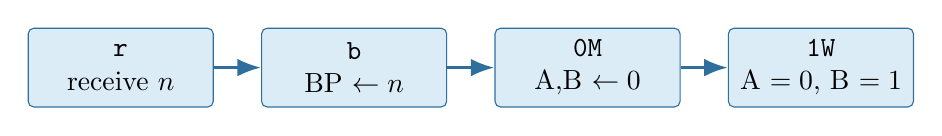
\begin{tikzpicture}[node distance=6mm]
  \node[process] (r) {\op{r}\\receive \(n\)};
  \node[process, right=of r] (b) {\op{b}\\BP \(\leftarrow n\)};
  \node[process, right=of b] (z) {\op{0}\op{M}\\A,B \(\leftarrow0\)};
  \node[process, right=of z] (o) {\op{1}\op{W}\\A \(=0\), B \(=1\)};
  \draw[flow] (r) -- (b);
  \draw[flow] (b) -- (z);
  \draw[flow] (z) -- (o);
\end{tikzpicture}
\end{center}

\begin{center}
\small
\begin{tabular}{c|c|c|c|p{6.4cm}}
  \toprule
  \textbf{Just executed} & \reg{A} & \reg{B} & \reg{BP} & \textbf{Why}\\
  \midrule
  nothing & 0 & 0 & 0 & All registers start at zero.\\
  \op{r} & \(n\) & 0 & 0 & Input arrives in the main hand.\\
  \op{b} & \(n\) & 0 & \(n\) & Save the loop count in BP.\\
  \op{0} & 0 & 0 & \(n\) & Start constructing the Fibonacci pair.\\
  \op{M} & 0 & 0 & \(n\) & Copy \(0\) into B.\\
  \op{1} & 1 & 0 & \(n\) & Temporarily put \(1\) in A.\\
  \op{W} & 0 & 1 & \(n\) & Swap: now A \(=\Fib0\), B \(=\Fib1\).\\
  \bottomrule
\end{tabular}
\end{center}

\begin{keybox}
  \textbf{Why the apparently silly sequence \op{0 M 1 W}?}
  Constants only load \reg{A}; there is no ``put 1 directly in B.''
  So we first make B \(=0\), then load \(1\) into A, then swap.
  The result is the exact starting pair \((0,1)\).
\end{keybox}

\section{Phase B: the loop controller}

After initialization, \op{v} turns the man downward. Two rows later,
\op{>} turns him right. He arrives at \op{d} facing right.

\begin{center}
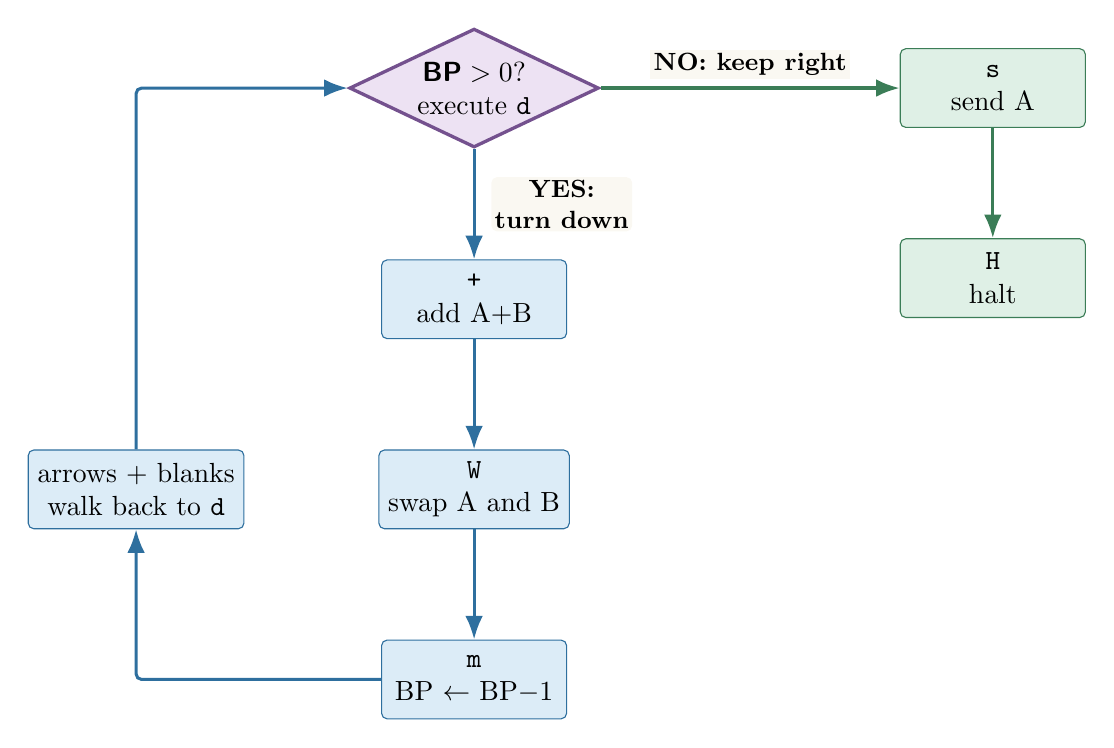
\begin{tikzpicture}[node distance=14mm and 15mm]
  \node[decision] (d) {\(\reg{BP}>0\)?\\execute \op{d}};
  \node[process, below=of d] (plus) {\op{+}\\add A+B};
  \node[process, below=of plus] (swap) {\op{W}\\swap A and B};
  \node[process, below=of swap] (dec) {\op{m}\\BP \(\leftarrow\) BP\(-1\)};
  \node[process, left=17mm of swap, minimum width=2.7cm] (walk) {
    arrows + blanks\\walk back to \op{d}
  };
  \node[process, right=38mm of d, fill=greenlight, draw=green] (send) {
    \op{s}\\send A
  };
  \node[process, below=of send, fill=greenlight, draw=green] (halt) {
    \op{H}\\halt
  };

  \draw[flow] (d) --
    node[arrowlabel, midway, right=2mm, font=\small\bfseries]
      {YES:\\turn down} (plus);
  \draw[flow] (plus) -- (swap);
  \draw[flow] (swap) -- (dec);
  \draw[flow] (dec.west) -| (walk.south);
  \draw[flow] (walk.north) |- (d.west);
  \draw[dataflow] (d) --
    node[arrowlabel, midway, above=1mm, font=\small\bfseries]
      {NO: keep right} (send);
  \draw[dataflow] (send) -- (halt);
\end{tikzpicture}
\end{center}

\textbf{At \op{d}, direction is part of the condition.}
The instruction does not contain an address or a label. It merely turns:

\begin{itemize}
  \item facing right + clockwise turn \(=\) face down, entering the blue loop;
  \item facing right + no turn \(=\) keep walking right, reaching \op{s H}.
\end{itemize}

That is geometric control flow. The man's heading replaces an ordinary
machine-code branch target.

\begin{warningbox}
  \textbf{Why test BP before performing the first addition?}
  Because \(n\) can be zero. If BP \(=0\), the machine must output
  \(\Fib0=0\) immediately. Entering the loop once would incorrectly output
  \(\Fib1=1\).
\end{warningbox}

\section{One lap: why \op{+ W} advances Fibonacci}

Assume the hands contain two neighboring Fibonacci numbers:
\[
  \reg{A}=\Fib{k},\qquad \reg{B}=\Fib{k+1}.
\]

\begin{center}
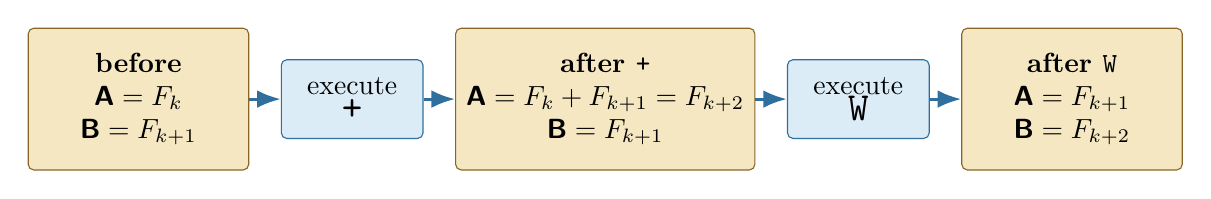
\begin{tikzpicture}[node distance=4mm]
  \node[register, minimum width=2.8cm, minimum height=1.8cm] (before) {
    \textbf{before}\\
    \(\reg{A}=\Fib{k}\)\\
    \(\reg{B}=\Fib{k+1}\)
  };
  \node[process, right=of before, minimum width=1.8cm] (plus) {
    execute\\[-1mm]\Large\op{+}
  };
  \node[register, right=of plus, minimum width=3.8cm,
    minimum height=1.8cm] (afterplus) {
    \textbf{after \op{+}}\\
    \(\reg{A}=\Fib{k}+\Fib{k+1}=\Fib{k+2}\)\\
    \(\reg{B}=\Fib{k+1}\)
  };
  \node[process, right=of afterplus, minimum width=1.8cm] (swap) {
    execute\\[-1mm]\Large\op{W}
  };
  \node[register, right=of swap, minimum width=2.8cm,
    minimum height=1.8cm] (afterswap) {
    \textbf{after \op{W}}\\
    \(\reg{A}=\Fib{k+1}\)\\
    \(\reg{B}=\Fib{k+2}\)
  };

  \draw[flow] (before) -- (plus);
  \draw[flow] (plus) -- (afterplus);
  \draw[flow] (afterplus) -- (swap);
  \draw[flow] (swap) -- (afterswap);
\end{tikzpicture}
\end{center}

Before the lap we hold \((\Fib{k},\Fib{k+1})\). After \op{+ W} we hold
\((\Fib{k+1},\Fib{k+2})\). That is the same shape with the index increased by
one. Then \op{m} decreases the remaining-lap count by one.

\begin{keybox}
  \textbf{This repeating statement is the whole proof:}
  \[
    \boxed{
      (\reg{A},\reg{B},\reg{BP})
      =
      (\Fib{k},\Fib{k+1},n-k)
    }
  \]
  It is true before the first lap with \(k=0\). One lap makes it true for
  \(k+1\). When BP reaches zero, \(n-k=0\), therefore \(k=n\), therefore
  \(\reg{A}=\Fib{n}\).
\end{keybox}

\section{Full worked example: input \texorpdfstring{\(n=5\)}{n=5}}

The expected answer is \(\Fib5=5\).

\subsection{Initialization}

\[
  (\reg{A},\reg{B},\reg{BP})=(0,1,5).
\]

\subsection{Five laps}

\begin{center}
\begin{tabular}{c|c|c|c|c}
  \toprule
  \textbf{At \op{d}} & \textbf{BP positive?} &
  \textbf{after \op{+}} & \textbf{after \op{W}} &
  \textbf{after \op{m}}\\
  \midrule
  \(A=0,B=1,BP=5\) & yes & \(A=1,B=1\) & \(A=1,B=1\) & \(BP=4\)\\
  \(A=1,B=1,BP=4\) & yes & \(A=2,B=1\) & \(A=1,B=2\) & \(BP=3\)\\
  \(A=1,B=2,BP=3\) & yes & \(A=3,B=2\) & \(A=2,B=3\) & \(BP=2\)\\
  \(A=2,B=3,BP=2\) & yes & \(A=5,B=3\) & \(A=3,B=5\) & \(BP=1\)\\
  \(A=3,B=5,BP=1\) & yes & \(A=8,B=5\) & \(A=5,B=8\) & \(BP=0\)\\
  \(A=5,B=8,BP=0\) & \textbf{no} &
  \multicolumn{3}{c}{walk right to \op{s}; send \(A=5\)}\\
  \bottomrule
\end{tabular}
\end{center}

\begin{center}
\small\textbf{Each arrow is one lap: execute \op{+ W m}.}\par\medskip
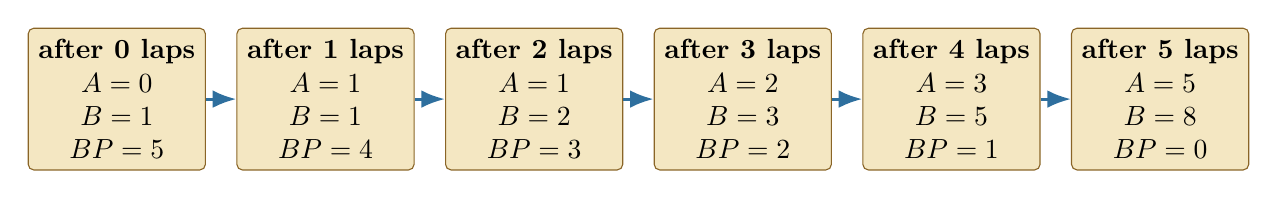
\begin{tikzpicture}[node distance=5mm]
  \foreach \k/\aval/\bval/\bpval in {
    0/0/1/5,
    1/1/1/4,
    2/1/2/3,
    3/2/3/2,
    4/3/5/1,
    5/5/8/0
  }{
    \node[
      register,
      minimum width=2.25cm,
      minimum height=1.8cm
    ] (s\k) at ({\k*2.65},0) {
      \textbf{after \k\ laps}\\
      \(A=\aval\)\\
      \(B=\bval\)\\
      \(BP=\bpval\)
    };
  }
  \foreach \k in {0,...,4}{
    \pgfmathtruncatemacro{\next}{\k+1}
    \draw[flow] (s\k.east) -- (s\next.west);
  }
\end{tikzpicture}
\end{center}

\begin{bluebox}
  Notice the ``extra'' \(8\) in \reg{B}. It is not a mistake.
  After five laps the pair is \((\Fib5,\Fib6)=(5,8)\).
  The problem asks for \(\Fib5\), so the machine correctly sends \reg{A},
  not \reg{B}.
\end{bluebox}

\section{Where the time goes}

For the validated machine:
\[
  \text{ticks}(n)=14+12n.
\]

The constant 14 covers input arrival, initialization, the final BP test,
sending, and output-pipe travel. Every additional Fibonacci lap costs 12
ticks:

\begin{center}
\begin{tabular}{l|r}
  \toprule
  \textbf{Part of one lap} & \textbf{ticks}\\
  \midrule
  Execute \op{d}, \op{+}, \op{W}, \op{m} & 4\\
  Execute the turn cells \op{<}, \op{\string^}, \op{>} & 3\\
  Walk over five blank cells & 5\\
  \midrule
  Total & 12\\
  \bottomrule
\end{tabular}
\end{center}

Blank corridors cost time. They are not visually exciting, but the man must
execute each blank as a no-op and move across it.

\clearpage
\section{Why there is no relay room here}

Your observation about relay rooms is correct:

\begin{warningbox}
  A legal pipe must end at a room different from the room where it began.
  Therefore one room cannot send a pipe directly back into itself.
\end{warningbox}

\begin{center}
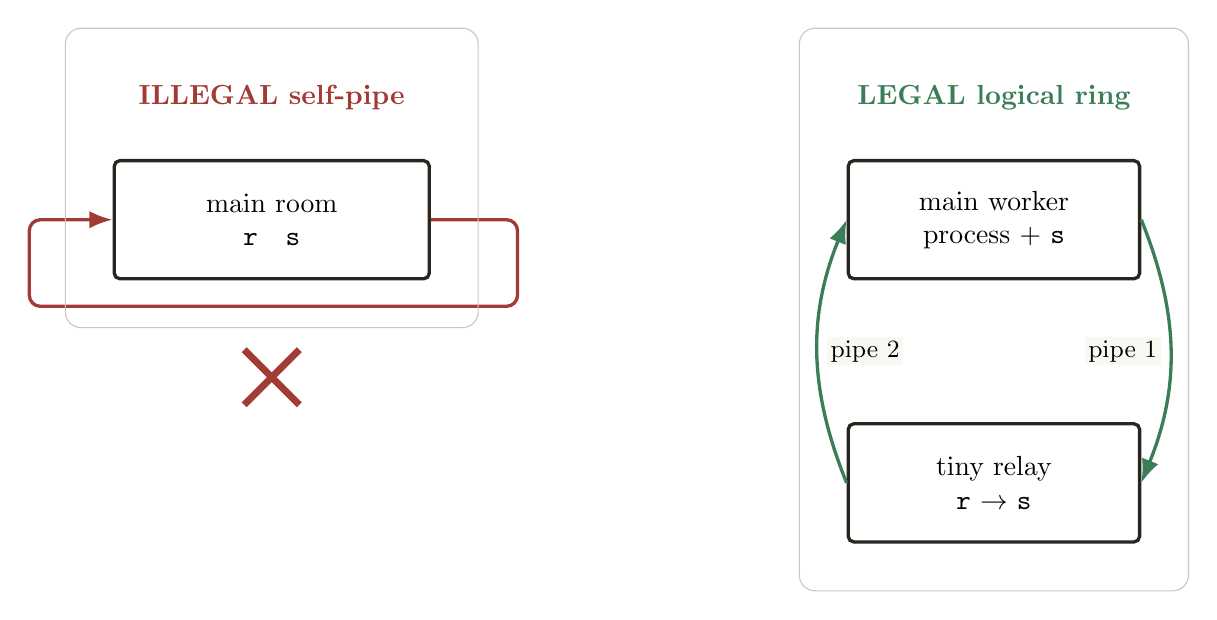
\begin{tikzpicture}[node distance=10mm]
  % Illegal half.
  \node[font=\bfseries, text=red] (badtitle) {ILLEGAL self-pipe};
  \node[room, below=5mm of badtitle, minimum width=4cm] (badmain) {
    main room\\
    \op{r}\quad\op{s}
  };
  \draw[-{Latex}, red, very thick, rounded corners=4pt]
    (badmain.east) -- ++(1.1,0) -- ++(0,-1.1) --
    ++(-6.2,0) -- ++(0,1.1) -- (badmain.west);
  \draw[red, line width=2.5pt]
    ($(badmain)+(0,-2.0)$) ++(-0.35,-0.35) -- ++(0.7,0.7);
  \draw[red, line width=2.5pt]
    ($(badmain)+(0,-2.0)$) ++(-0.35,0.35) -- ++(0.7,-0.7);

  % Legal half.
  \node[font=\bfseries, text=green, right=55mm of badtitle] (goodtitle) {
    LEGAL logical ring
  };
  \node[room, below=5mm of goodtitle, minimum width=3.7cm] (main) {
    main worker\\
    process + \op{s}
  };
  \node[room, below=18mm of main, minimum width=3.7cm] (relay) {
    tiny relay\\
    \op{r}\ \(\rightarrow\)\ \op{s}
  };
  \draw[dataflow, bend left=22] (main.east) to
    node[arrowlabel, left=1mm]{pipe 1} (relay.east);
  \draw[dataflow, bend left=22] (relay.west) to
    node[arrowlabel, right=1mm]{pipe 2} (main.west);
  \node[fit=(badtitle)(badmain), inner sep=6mm, draw=line,
    rounded corners=2mm] {};
  \node[fit=(goodtitle)(main)(relay), inner sep=6mm, draw=line,
    rounded corners=2mm] {};
\end{tikzpicture}
\end{center}

The relay man receives a value from pipe 1 and sends it into pipe 2.
Together, the two legal pipes behave like one feedback FIFO.

\textbf{Fibonacci does not need that memory.} At any moment, the future
depends only on the two most recent values. Those fit in \reg{A} and \reg{B},
so a relay would only make the program larger and slower.

\section{Common wrong versions}

\begin{enumerate}
  \item \textbf{Starting with A=1, B=1.}\\
        Then zero laps outputs 1, so \(n=0\) is wrong. Start with \((0,1)\).

  \item \textbf{Doing the body before testing BP.}\\
        Again, \(n=0\) incorrectly performs one lap. Test first.

  \item \textbf{Using only \op{+}, without \op{W}.}\\
        After addition the registers are
        \((\Fib{k+2},\Fib{k+1})\), in the wrong order for the next addition.
        Swap restores the invariant.

  \item \textbf{Sending B.}\\
        After \(n\) laps, B is \(\Fib{n+1}\). The requested answer is in A.

  \item \textbf{Trying to read BP into A.}\\
        No such instruction exists. Arrange the algorithm so BP is used only
        for control.

  \item \textbf{Forgetting that arrows consume ticks.}\\
        Direction cells and blank corridors are part of the running time.

  \item \textbf{Letting the man walk into a wall.}\\
        That is a program error, not an implicit halt. Use \op{H}.
\end{enumerate}

\clearpage
\section{How to watch it yourself}

\subsection{In the archived web editor}

After the accompanying site change is published:

\begin{center}
  \url{https://tarstars.github.io/problems/fibonacci/editor/}
\end{center}

Paste the program, enter an input such as \(5\), put \(5\) in the expected
output box, choose a slow speed, and use \textbf{next} one tick at a time.
Watch these three things:

\begin{enumerate}
  \item the man blocks briefly on \op{r} until input reaches him;
  \item \reg{A}/\reg{B} become \(0/1\), then walk through neighboring
        Fibonacci pairs;
  \item at BP \(=0\), \op{d} no longer turns the man downward.
\end{enumerate}

\subsection{With the repository simulator}

\begin{Verbatim}[fontsize=\small]
uv run python - <<'PY'
import json
from pathlib import Path
from littleman.judge import judge_problem

program = Path("docs/littleman_fibonacci.man").read_text()
problem = {
    "slug": "fibonacci",
    "scoring": "footprint-tick",
    "tickCap": 5000,
    "publicTestData": [
        {"name": "five", "in": ["5"], "out": ["5"]},
    ],
}
print(judge_problem(program, problem))
PY
\end{Verbatim}

\section{Validation evidence}

The exact checked-in \texttt{.man} file used by this document passed:

\begin{center}
\begin{tabular}{r|r|r}
  \toprule
  \(n\) & expected/observed \(\Fib n\) & ticks\\
  \midrule
  0  & 0 & 14\\
  1  & 1 & 26\\
  2  & 1 & 38\\
  5  & 5 & 74\\
  10 & 55 & 134\\
  20 & 6,765 & 254\\
  50 & 12,586,269,025 & 614\\
  92 & 7,540,113,804,746,346,429 & 1,118\\
  \bottomrule
\end{tabular}
\end{center}

Its occupied bounding box is \(24\times9\), so its contest footprint would be
\(24^2=576\). This is a teaching layout, not a size-optimized contest entry.
The generous room makes the loop visually obvious.

\clearpage
\section{Your compact program: before and after}

Now that the roomy teaching version is understandable, we can look at your
actual contest-sized versions. They compute the same function with the same
three-register invariant. The difference is how tightly the man's useful
work is arranged inside the worker room.

\begin{center}
\begin{minipage}[t]{0.47\textwidth}
  \centering
  {\large\bfseries\textcolor{red}{Your original program}}\par
  \smallskip
  \textcolor{muted}{Correct, but not yet optimized}
  \begin{plainbox}
\begin{Verbatim}[fontsize=\small]
+-------+
|@rb1M0v|
| v   <<|
| >dsHW |
|  >m+^ |
+-------+
^<+-++-+v
  |I||O|<
  +-++-+
\end{Verbatim}
  \end{plainbox}
\end{minipage}
\hfill
\begin{minipage}[t]{0.47\textwidth}
  \centering
  {\large\bfseries\textcolor{green}{Your optimized program}}\par
  \smallskip
  \textcolor{muted}{Same algorithm, shorter walking route}
  \begin{plainbox}
\begin{Verbatim}[fontsize=\small]
+-------+
|@rb1Wv |
|  Hsa<<|
|    m W|
|    >+^|
+-------+
^<+-++-+v
  |I||O|<
  +-++-+
\end{Verbatim}
  \end{plainbox}
\end{minipage}
\end{center}

\begin{warningbox}
  \textbf{The short pipes are legal, but they are not one-cell pipes.}
  Each pipe contains two pipe characters between different rooms. The rule
  forbids a pipe from returning to its own starting room; neither program
  does that.
\end{warningbox}

\subsection{The measured result}

The validation corpus was
\(n\in\{0,1,2,5,10,20,50,92\}\). Both programs produced the expected
Fibonacci number in every case.

\begin{center}
\begin{tabularx}{\textwidth}{
  >{\raggedright\arraybackslash}X
  >{\centering\arraybackslash}p{2.1cm}
  >{\centering\arraybackslash}p{2.8cm}
  >{\centering\arraybackslash}p{2.2cm}
  >{\centering\arraybackslash}p{2.2cm}}
  \toprule
  \textbf{Version} & \textbf{Bounding box} & \textbf{Tick formula}
    & \textbf{Average ticks} & \textbf{Score}\\
  \midrule
  Original & \(9\times9\) & \(17+12n\) & 287 & 23,247\\
  Optimized & \(9\times9\) & \(10+8n\) & 190 & 15,390\\
  \bottomrule
\end{tabularx}
\end{center}

\begin{keybox}
  \centering
  \Large
  The footprint stays \(9^2=81\), but the score falls by
  \[
    \frac{23\,247-15\,390}{23\,247}\times100\%
    =\boxed{33.80\%}.
  \]
  \normalsize
  This improvement comes entirely from optimizing the program
  \emph{inside} the worker room. Outer component packing cannot reduce this
  particular pair any further unless it also changes the \(9\times9\)
  bounding square.
\end{keybox}

\clearpage
\section{Exactly why the optimized program is faster}

\subsection[Optimization 1: prepare A and B in four operations]{
  Optimization 1: prepare \((A,B)=(0,1)\) in four operations
}

All registers begin at zero. Your original setup is:
\[
  \underbrace{\op{r}\ \op{b}\ \op{1}\ \op{M}\ \op{0}}_{\text{five
  operations}}.
\]

\begin{center}
\begin{tabular}{c|c|c|c|l}
  \toprule
  \textbf{after} & \reg{A} & \reg{B} & \reg{BP} & \textbf{meaning}\\
  \midrule
  \op{r} & \(n\) & 0 & 0 & receive the input\\
  \op{b} & \(n\) & 0 & \(n\) & save the loop count\\
  \op{1} & 1 & 0 & \(n\) & put 1 in A\\
  \op{M} & 1 & 1 & \(n\) & copy A to B\\
  \op{0} & 0 & 1 & \(n\) & put 0 in A\\
  \bottomrule
\end{tabular}
\end{center}

The optimized setup is:
\[
  \underbrace{\op{r}\ \op{b}\ \op{1}\ \op{W}}_{\text{four operations}}.
\]
After \op{1}, the state is \((A,B,BP)=(1,0,n)\). The initial zero already
waiting in B is useful: \op{W} swaps the two hands and immediately gives
\((0,1,n)\). Thus \op{W} replaces the two-operation pair \op{M}\op{0}.

\begin{center}
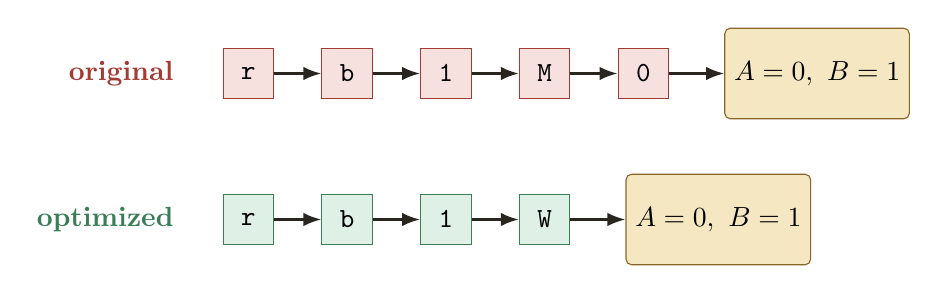
\begin{tikzpicture}[node distance=5mm and 6mm]
  \node[opcell, fill=redlight, draw=red] (or) {\op{r}};
  \node[opcell, fill=redlight, draw=red, right=of or] (ob) {\op{b}};
  \node[opcell, fill=redlight, draw=red, right=of ob] (o1) {\op{1}};
  \node[opcell, fill=redlight, draw=red, right=of o1] (om) {\op{M}};
  \node[opcell, fill=redlight, draw=red, right=of om] (o0) {\op{0}};

  \node[opcell, fill=greenlight, draw=green, below=12mm of or] (nr) {\op{r}};
  \node[opcell, fill=greenlight, draw=green, right=of nr] (nb) {\op{b}};
  \node[opcell, fill=greenlight, draw=green, right=of nb] (n1) {\op{1}};
  \node[opcell, fill=greenlight, draw=green, right=of n1] (nw) {\op{W}};

  \foreach \a/\b in {or/ob,ob/o1,o1/om,om/o0,nr/nb,nb/n1,n1/nw}{
    \draw[-{Latex[length=2.3mm]}, line width=0.9pt, draw=ink]
      (\a.east) -- (\b.west);
  }
  \node[left=5mm of or, text=red, font=\bfseries] {original};
  \node[left=5mm of nr, text=green, font=\bfseries] {optimized};
  \node[right=7mm of o0, register, minimum width=2.3cm]
    (ostate) {\(A=0,\ B=1\)};
  \node[right=7mm of nw, register, minimum width=2.3cm]
    (nstate) {\(A=0,\ B=1\)};
  \draw[-{Latex[length=2.3mm]}, line width=0.9pt, draw=ink]
    (o0.east) -- (ostate.west);
  \draw[-{Latex[length=2.3mm]}, line width=0.9pt, draw=ink]
    (nw.east) -- (nstate.west);
\end{tikzpicture}
\end{center}

\subsection{Optimization 2: fold the control path around the arithmetic}

Both versions repeat the same useful work:

\begin{center}
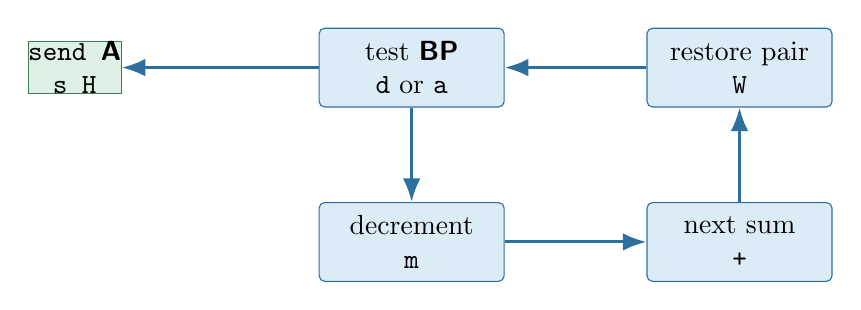
\begin{tikzpicture}[node distance=12mm and 18mm]
  \node[process] (test) {test \reg{BP}\\\op{d} or \op{a}};
  \node[process, below=of test] (dec) {decrement\\\op{m}};
  \node[process, right=of dec] (add) {next sum\\\op{+}};
  \node[process, above=of add] (swap) {restore pair\\\op{W}};
  \draw[flow] (test) -- (dec);
  \draw[flow] (dec) -- (add);
  \draw[flow] (add) -- (swap);
  \draw[flow] (swap) -- (test);
  \node[exitcell, align=center, left=25mm of test] (send) {
    send \reg{A}\\\op{s}\ \op{H}
  };
  \draw[flow] (test) -- (send);
\end{tikzpicture}
\end{center}

\begin{plainbox}
  The two arrows leaving the test have no text drawn over them, so read this
  separate legend: when \(\reg{BP}>0\), the man turns into the loop; when
  \(\reg{BP}=0\), he walks straight to \op{s} and \op{H}.
\end{plainbox}

In the original room, \op{d} is approached while walking right. A positive
BP makes \op{d} turn clockwise, so the man turns downward. In the optimized
room, \op{a} is approached while walking left. A positive BP makes \op{a}
turn counter-clockwise; from a leftward heading, that also means downward.
For BP \(=0\), both instructions continue straight toward the send cell.

\clearpage
\subsection{Optimization 3: remove walking-only cells from every lap}

Here is one complete loop, written in the exact order in which the man
executes the cells:

\begin{center}
\begin{tabularx}{\textwidth}{
  >{\raggedright\arraybackslash}p{2.3cm}
  >{\raggedright\arraybackslash}X
  >{\centering\arraybackslash}p{1.5cm}}
  \toprule
  \textbf{Version} & \textbf{one positive-BP lap} & \textbf{ticks}\\
  \midrule
  Original &
  \(\op{d},\op{>},\op{m},\op{+},\op{\string^},\op{W},
    \op{<},\text{blank},\text{blank},\text{blank},\op{v},\op{>}\)
  & 12\\
  Optimized &
  \(\op{a},\op{m},\op{>},\op{+},\op{\string^},\op{W},
    \op{<},\op{<}\)
  & 8\\
  \bottomrule
\end{tabularx}
\end{center}

\begin{center}
\begin{tabular}{l|r|r|r}
  \toprule
  \textbf{Cells executed per lap} & \textbf{Original}
    & \textbf{Optimized} & \textbf{saved}\\
  \midrule
  Useful operations: branch, \op{m}, \op{+}, \op{W} & 4 & 4 & 0\\
  Direction cells & 5 & 4 & 1\\
  Blank cells & 3 & 0 & 3\\
  \midrule
  Total & 12 & 8 & 4\\
  \bottomrule
\end{tabular}
\end{center}

The arithmetic itself is not cheaper. The man still must test BP, decrement
BP, add the two Fibonacci values, and swap them. The gain comes from arranging
those operations so that the return journey is shorter and contains no
blank cells.

\subsection{Where the two formulas come from}

\begin{center}
\begin{tabular}{l|r|r}
  \toprule
  \textbf{Part} & \textbf{Original} & \textbf{Optimized}\\
  \midrule
  Register preparation & 5 & 4\\
  Walk from preparation to the branch & 8 & 2\\
  Final branch, send, halt, and output travel & 4 & 4\\
  \midrule
  Fixed cost, even for \(n=0\) & 17 & 10\\
  Cost of each Fibonacci lap & 12 & 8\\
  \bottomrule
\end{tabular}
\end{center}

Therefore:
\[
  T_{\text{original}}(n)=17+12n,
  \qquad
  T_{\text{optimized}}(n)=10+8n.
\]

\begin{center}
\begin{tabular}{r|r|r|r}
  \toprule
  \(n\) & \(\Fib n\) & \textbf{original ticks}
    & \textbf{optimized ticks}\\
  \midrule
  0  & 0 & 17 & 10\\
  1  & 1 & 29 & 18\\
  2  & 1 & 41 & 26\\
  5  & 5 & 77 & 50\\
  10 & 55 & 137 & 90\\
  20 & 6,765 & 257 & 170\\
  50 & 12,586,269,025 & 617 & 410\\
  92 & 7,540,113,804,746,346,429 & 1,121 & 746\\
  \bottomrule
\end{tabular}
\end{center}

\begin{bluebox}
  \textbf{The general optimization lesson:}
  first minimize the useful instruction sequence under the room's register
  contract; then place those instructions so the man reaches them with the
  fewest arrows and blanks; finally pack and reroute whole rooms. Your
  Fibonacci improvement wins at the second level while keeping the outer
  layout unchanged.
\end{bluebox}

\begin{keybox}
  \centering
  \Large\bfseries
  If you remember only one sentence, remember this:

  \vspace{2mm}
  \normalsize
  A holds the answer for the current index, B holds the answer for the next
  index, BP counts how many index advances remain, and one geometric lap
  performs exactly one advance.
\end{keybox}

\vfill
\begin{center}
  {\color{gold}\rule{0.7\textwidth}{1.3pt}}\\[4mm]
  \small
  Source program:
  \texttt{docs/littleman\_fibonacci.man}\\
  Reproducible document source:
  \texttt{docs/littleman\_fibonacci\_illustrated.tex}
\end{center}

\end{document}
